\documentclass[boxes,pages]{homework}

\name{Nate Stemen}
\studentid{20906566}
\email{nate.stemen@uwaterloo.ca}
\term{Fall 2020}
\course{Numerical Analysis}
\courseid{AMATH 740}
\hwnum{C}
\duedate{Mon, Dec 7, 2020 5:00 PM}

\hwname{Computational Assignment}

\usepackage{physics}
% \usepackage{cleveref}
\usepackage{listings}
\usepackage{xcolor}
\usepackage{graphicx}
\usepackage{caption}

\definecolor{codegreen}{rgb}{0,0.6,0}
\definecolor{codegray}{rgb}{0.5,0.5,0.5}
\definecolor{codepurple}{rgb}{0.58,0,0.82}
\definecolor{backcolour}{rgb}{0.95,0.95,0.92}

\lstloadlanguages{Python}
\lstdefinestyle{mystyle}{
  language=Python,
  backgroundcolor=\color{backcolour},
  commentstyle=\color{codegreen},
  keywordstyle=\color{magenta},
  numberstyle=\tiny\color{codegray},
  stringstyle=\color{codepurple},
  basicstyle=\ttfamily\footnotesize,
  numbers=left,
  numbersep=5pt,
  showstringspaces=false,
	breaklines=true,
	title=\lstname
}
\lstset{style=mystyle}

\begin{document}

\problemnumber{3}

\begin{problem}
Adaptive RK45 method.
\end{problem}

\begin{solution}
	First, the code. Note: I put everything in one file because it was simple enough that breaking it into multiple files felt unnecessary, and overcomplicated.
	\lstinputlisting[language=Python]{adaptiveRK.py}
	And here's the output of \verb|adaptiveRK.py|:
	\begin{verbatim}Total iterations:     182
Function Evaluations: 182 * 6 = 1092
Smallest step taken:  0.020509068135583064
Total evaluations needed for all small steps: 5851.070326876577\end{verbatim}
	From here we can see that the adaptive method is \emph{much} more efficient than had we used a fixed step length method with this smallest step length. Sweet!
	And now the plots:
	\begin{center}
		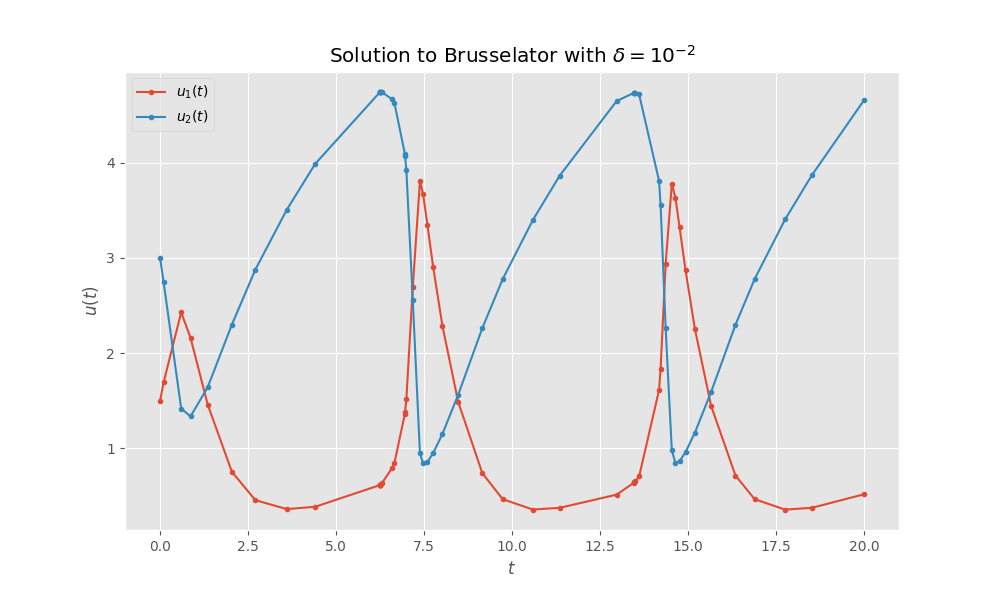
\includegraphics[width=0.9\textwidth]{10-2.png}
		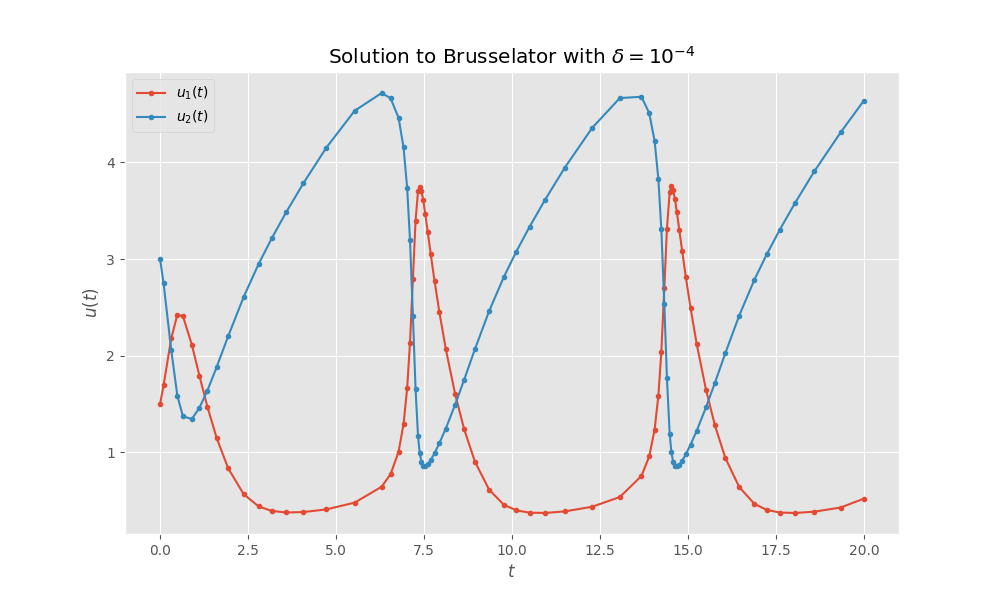
\includegraphics[width=0.9\textwidth]{10-4.png}
		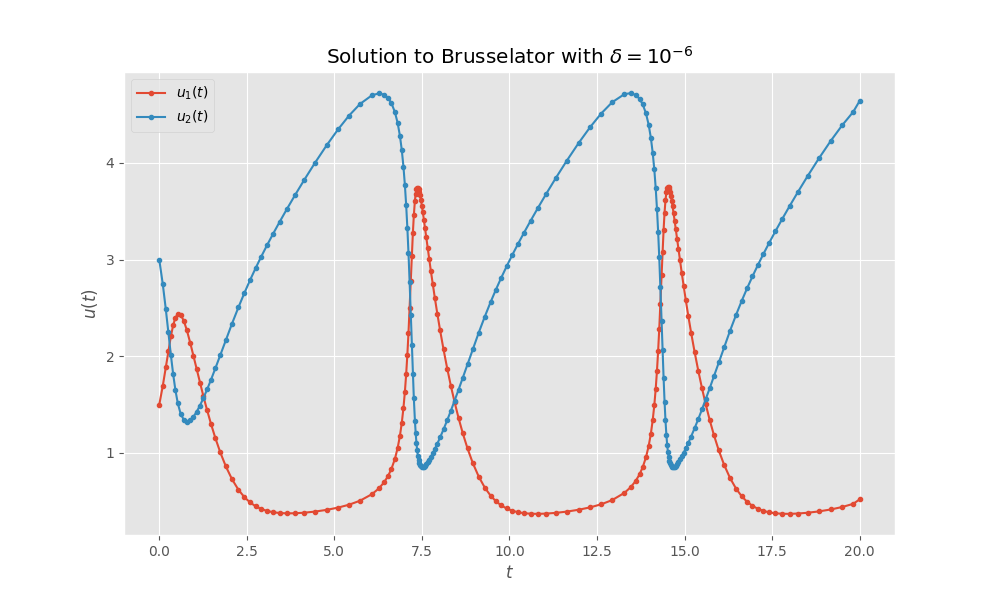
\includegraphics[width=0.9\textwidth]{10-6.png}
		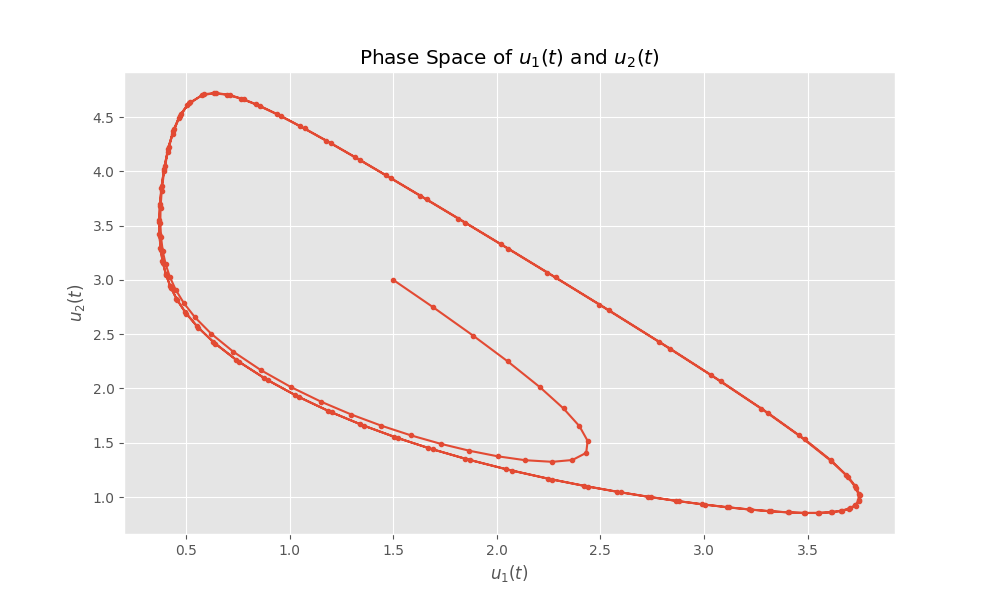
\includegraphics[width=0.9\textwidth]{phase-space.png}
	\end{center}
	We see in the phase space plot that the solution very quickly approaches an orbit, and then stays on that orbit for what seems like the rest of the evolution.

\end{solution}


\end{document}